% \documentclass[aspectratio=169, 11pt]{beamer}
\documentclass[aspectratio=169, 11pt, handout]{beamer}

% Meeting 8 lecture slides. Running case: Wen's rate decision at Meridian Hotels (cases/caseB-meridian, Meeting 8
% releases R1 to R5). The notes' worked example (QuickBite) is deliberately not reproduced here.
% Shared with notes.tex: estimands, assumptions, notation, the statement of each Result, the order of topics.
% Block A follows notes Sections 1.1 to 1.3 (through the product of errors); block B follows the rest of Section 1.3
% (inference, repeated splits, learners) and Sections 1.4 to 1.6.
% Every number is checked by shared/checks/slides08_check.py.

% ── Theme ──
\usetheme{Madrid}
\usecolortheme{default}
\setbeamertemplate{navigation symbols}{}
\setbeamertemplate{footline}{%
  \leavevmode\hbox{%
    \begin{beamercolorbox}[wd=.333333\paperwidth,ht=2.5ex,dp=1ex,center]{author in head/foot}%
      \usebeamerfont{author in head/foot}\insertshortauthor
    \end{beamercolorbox}%
    \begin{beamercolorbox}[wd=.333333\paperwidth,ht=2.5ex,dp=1ex,center]{title in head/foot}%
      \usebeamerfont{title in head/foot}\insertshorttitle
    \end{beamercolorbox}%
    \begin{beamercolorbox}[wd=.333333\paperwidth,ht=2.5ex,dp=1ex,right]{date in head/foot}%
      \usebeamerfont{date in head/foot}\insertframenumber{} / \inserttotalframenumber\hspace*{2ex}
    \end{beamercolorbox}}}

% ── Packages ──
\usepackage{amsmath,amssymb}
\usepackage{booktabs}
\usepackage{xcolor}
\usepackage{colortbl}
\usepackage{tikz}
\usetikzlibrary{arrows.meta, positioning, calc}
\usepackage{pgfplots}
\pgfplotsset{compat=1.18}

% ── Colours: the notes' palette (shared/coursenotes.sty), so a Result looks the same in both ──
\definecolor{sbgreen}{HTML}{00704A}
\definecolor{noteblue}{HTML}{2060A0}
\definecolor{warnred}{HTML}{B42318}
\definecolor{extgrey}{HTML}{6B7280}
\definecolor{boxgrey}{HTML}{F3F5F8}
\definecolor{bluetint}{HTML}{EEF3FA}
\definecolor{greentint}{HTML}{EEF6F2}
\definecolor{redtint}{HTML}{FCF1F0}

% ── Notation: same macros as the notes (shared/coursenotes.sty, shared/notation.tex) ──
\newcommand{\E}{\mathbb{E}}
\newcommand{\Var}{\operatorname{Var}}
\newcommand{\Cov}{\operatorname{Cov}}
\newcommand{\SE}{\operatorname{SE}}
\newcommand{\indep}{\perp\!\!\!\perp}
\newcommand{\hatt}{\hat{\tau}}
\newcommand{\ATE}{\text{ATE}}
\newcommand{\ATT}{\text{ATT}}
\newcommand{\ATU}{\text{ATU}}

% ── Boxes: same number, title and wording as the notes; proofs stay in the notes ──
\newenvironment{result}[2]{%
  \setbeamercolor{block title}{bg=sbgreen,fg=white}\setbeamercolor{block body}{bg=greentint,fg=black}%
  \begin{block}{Result #1 (#2)}}{\end{block}}
\newenvironment{assumption}[2]{%
  \setbeamercolor{block title}{bg=noteblue,fg=white}\setbeamercolor{block body}{bg=bluetint,fg=black}%
  \begin{block}{Assumption #1 (#2)}}{\end{block}}
\newenvironment{defbox}[1]{%
  \setbeamercolor{block title}{bg=extgrey,fg=white}\setbeamercolor{block body}{bg=boxgrey,fg=black}%
  \begin{block}{Definition: #1}}{\end{block}}
\newenvironment{pitfall}[1]{%
  \setbeamercolor{block title}{bg=warnred,fg=white}\setbeamercolor{block body}{bg=redtint,fg=black}%
  \begin{block}{Pitfall: #1}}{\end{block}}

% Step labels for the course spine
\newcommand{\spinestep}[1]{\textcolor{sbgreen}{\textbf{#1}}}

% ── Title ──
\title[Meeting 8]{Meeting 8: Double Machine Learning}
\subtitle{Flexible controls without biased answers: Wen's rate decision}
\author{Zhikun Lu}
\date{}

\begin{document}

% ====================================================================
\begin{frame}
\titlepage
\end{frame}

% ====================================================================
\begin{frame}{Today}

\begin{columns}[T]
\begin{column}{0.48\textwidth}
\textbf{Block A: DML I}
\begin{itemize}
  \item An 8\% rate rise and its break-even
  \item Six nights: pooled versus within category
  \item The partially linear model and its assumptions
  \item Residualization (FWL); what $\theta$ averages
  \item Why plug-in machine learning fails
  \item Cross-fitting and the product of errors
  \item The price elasticity at Meridian
\end{itemize}
\end{column}
\begin{column}{0.48\textwidth}
\textbf{Block B: DML II}
\begin{itemize}
  \item Inference: clustered SEs and repeated splits
  \item Choosing the nuisance learners
  \item Overlap with a continuous rate; a local slope
  \item The interactive model and the AIPW score
  \item DML for the CATE
  \item Sensitivity: omitted-variable bounds and benchmarking
\end{itemize}
\end{column}
\end{columns}
\end{frame}

% ====================================================================
\section{Block A: DML I}
% ====================================================================

% [RELEASE R1: the proposal and the six comparable nights]
\begin{frame}{Meridian Hotels: The Proposal}

Wen is commercial director of Meridian Hotels, a group of 80 properties.

\bigskip

A revenue management (RM) system sets the rate for every hotel-night from forecast demand, competitor rates, booking pace, and the event calendar. No human sets these rates night by night. The system is an automated decision-maker, and, as in Meeting 7, its decisions are what the analysis must adjust for.

\bigskip

On her desk is a proposal from sales to raise midweek premium rates by \textbf{8\%} across the portfolio. Their evidence is the RM system's own reporting: nights with higher rates sell more rooms. Sales reads this as strong demand and a system that is under-pricing.

\bigskip

\begin{itemize}
  \item Current midweek premium rate \textyen 800; variable cost \textyen 200 per occupied room.
  \item Three years of logs: 80 hotels $\times$ 1{,}095 nights $=$ 87{,}600 hotel-nights, with 47 recorded signals per night.
\end{itemize}
\end{frame}

% ====================================================================
\begin{frame}{The Number That Decides It}

Contribution per occupied room is the rate less the variable cost:
\[
800 - 200 = \text{\textyen}\,600 \quad\longrightarrow\quad 864 - 200 = \text{\textyen}\,664, \quad \text{up } 10.7\%.
\]

The rise pays only if bookings fall by less than $1 - 600/664 = 9.6\%$.

\bigskip

Write $\theta$ for the \textbf{elasticity} of bookings with respect to the rate, the \% change in bookings from a 1\% change in the rate. An 8\% rise multiplies bookings by $1.08^{\theta}$, so it pays if and only if $1.08^{\theta} \times 664 > 600$:

\begin{alertblock}{Break-even elasticity}
\[
\theta^{\ast} = \frac{\ln(600/664)}{\ln 1.08} = -1.32 .
\]
\end{alertblock}

\medskip

The rise pays if demand is \emph{less} elastic than this, $\theta > -1.32$. Every estimate today is held against $-1.32$.
\end{frame}

% ====================================================================
\begin{frame}{Six Comparable Nights}

\begin{columns}[c]
\begin{column}{0.44\textwidth}
Six nights from one hotel, with rate $D$ and bookings $Y$:

\begin{center}
\small
\begin{tabular}{clrr}
\toprule
\textbf{Night} & \textbf{Category} & $D$ & $Y$ \\
\midrule
1 & Standard & 30 & 110 \\
2 & Standard & 40 & 100 \\
3 & Standard & 50 & \phantom{0}90 \\
4 & Premium  & 70 & 210 \\
5 & Premium  & 80 & 200 \\
6 & Premium  & 90 & 190 \\
\bottomrule
\end{tabular}
\end{center}

\end{column}
\begin{column}{0.54\textwidth}
\begin{center}
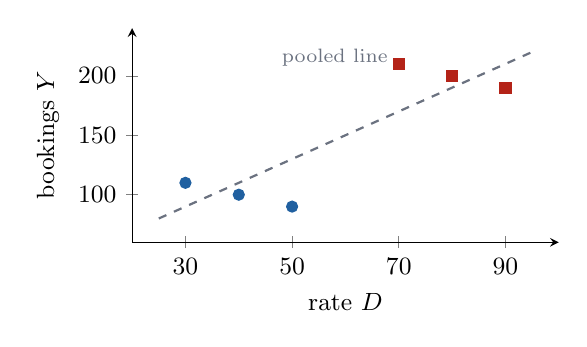
\begin{tikzpicture}
\begin{axis}[width=7.0cm, height=4.3cm, xlabel={rate $D$}, ylabel={bookings $Y$}, axis lines=left,
  xmin=20, xmax=100, ymin=60, ymax=240, xtick={30,50,70,90}, ytick={100,150,200}, label style={font=\small}, tick label style={font=\small}]
\addplot[only marks, mark=*, mark size=2pt, color=noteblue] coordinates {(30,110) (40,100) (50,90)};
\addplot[only marks, mark=square*, mark size=2pt, color=warnred] coordinates {(70,210) (80,200) (90,190)};
\addplot[thick, extgrey, dashed, domain=25:95] {30 + 2*x};
\node[font=\scriptsize, extgrey] at (axis cs:58,215) {pooled line};
\end{axis}
\end{tikzpicture}
\end{center}
\end{column}
\end{columns}

\medskip

With means $\bar D = 60$ and $\bar Y = 150$, the pooled slope of bookings on rate is
\[
\hat b_{\text{pooled}} = \frac{\sum_i (D_i - 60)(Y_i - 150)}{\sum_i (D_i - 60)^2} = \frac{5{,}600}{2{,}800} = \textcolor{warnred}{+2.0} .
\]
Read at face value, every \textyen 10 on the rate brings 20 more bookings. That is sales' case for the rise.
\end{frame}

% ====================================================================
% [RELEASE R2: the category means and the team's three sentences about the RM system]
\begin{frame}{Pooled, Then Within Category}

\begin{columns}[c]
\begin{column}{0.50\textwidth}
Subtract each category's means (40 and 100 for standard nights, 80 and 200 for premium):

\begin{center}
\small
\begin{tabular}{lrrrrrr}
\toprule
Night & 1 & 2 & 3 & 4 & 5 & 6 \\
\midrule
$\tilde D$ & $-10$ & 0 & 10 & $-10$ & 0 & 10 \\
$\tilde Y$ & 10 & 0 & $-10$ & 10 & 0 & $-10$ \\
\bottomrule
\end{tabular}
\end{center}
\[
\hat\theta = \frac{\sum_i \tilde D_i \tilde Y_i}{\sum_i \tilde D_i^2} = \frac{-400}{400} = \textcolor{sbgreen}{-1.0} .
\]
The same six nights give the opposite sign.
\end{column}
\begin{column}{0.46\textwidth}
\begin{center}
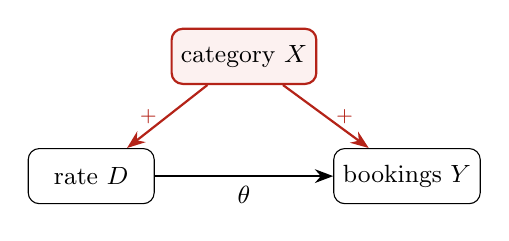
\begin{tikzpicture}[
    node distance=0.8cm and 0.2cm,
    v/.style={draw, rounded corners, minimum width=1.6cm, minimum height=0.7cm, font=\small},
    hid/.style={v, fill=redtint, draw=warnred, thick}
]
\node[hid] (X) {category $X$};
\node[v, below left=of X] (P) {rate $D$};
\node[v, below right=of X] (Q) {bookings $Y$};
\draw[-{Stealth}, warnred, thick] (X) -- node[left, font=\scriptsize] {$+$} (P);
\draw[-{Stealth}, warnred, thick] (X) -- node[right, font=\scriptsize] {$+$} (Q);
\draw[-{Stealth}, thick] (P) -- node[below, font=\small] {$\theta$} (Q);
\end{tikzpicture}
\end{center}
\end{column}
\end{columns}

\bigskip

The RM system prices premium nights high \emph{because} it forecasts high demand. Both arrows from $X$ are positive, so leaving $X$ out biases the slope upwards, here by enough to flip its sign. The $-1.0$ is in rooms per yuan; with logs on both sides the same slope is an elasticity.
\end{frame}

% ====================================================================
\begin{frame}{The Partially Linear Model}

With outcome $Y$ (log premium bookings), treatment $D$ (log rate), and controls $X$ (the 47 signals):
\[
Y = \theta D + g(X) + \varepsilon, \qquad \E[\varepsilon \mid D, X] = 0 .
\]
The model is linear in $D$, so $\theta$ is one number, the elasticity. It is unrestricted in $X$, so $g$ may be any function, as stepped as the RM rule. The \textbf{nuisance functions} are $\ell(X) = \E[Y \mid X]$ and $r(X) = \E[D \mid X]$.

\begin{assumption}{1.1}{Conditional mean independence}
$\E[\varepsilon \mid D, X] = 0$: given $X$, nothing left in the outcome moves with $D$.
\end{assumption}

\begin{assumption}{1.2}{Residual treatment variation}
$\E[\Var(D \mid X)] > 0$: treatment is not a deterministic function of $X$.
\end{assumption}

\smallskip
The first is Meeting 7's exchangeability for a continuous treatment. The second asks that the system did not price every night exactly by rule.
\end{frame}

% ====================================================================
\begin{frame}{What the Assumptions Say at Meridian}

What Wen's team says about the RM system:

\begin{center}
\small
\begin{tabular}{p{6.0cm}p{7.0cm}}
\toprule
\textbf{The team says} & \textbf{Which buys} \\
\midrule
``The RM system is the only thing setting rates.'' & No unrecorded input moves $D$ (Assumption 1.1). \\[0.4em]
``Every input it used is in the feed.'' & Nothing the system saw is missing from $X$ (Assumption 1.1). \\[0.4em]
``Rates still move for reasons unrelated to demand.'' & $\Var(D \mid X) > 0$: something is left to compare (Assumption 1.2). \\
\bottomrule
\end{tabular}
\end{center}

\medskip

\textbf{Measured as of the moment the rate was set.} Booking pace recorded after the rate posted, or a competitor index that reacts to Meridian's own rate, is partly caused by $D$: a mediator or a collider (Meeting 7), and a bad control. Every signal in $X$ must be time-stamped before the rate.

\medskip

A night priced exactly by the rule has $D - r(X) = 0$. It tells us nothing about $\theta$, however many such nights there are.
\end{frame}

% ====================================================================
\begin{frame}{Residualization}

\begin{result}{1.3}{Frisch--Waugh--Lovell in population form}
Under the model, $Y - \ell(X) = \theta\{D - r(X)\} + \varepsilon$, so
\[
  \theta = \frac{\E[(D - r(X))(Y - \ell(X))]}{\E[(D - r(X))^2]} .
\]
\end{result}

\medskip

\begin{itemize}
  \item $\tilde D = D - r(X)$: a night the system priced above or below what its own signals called for.
  \item $\tilde Y = Y - \ell(X)$: a night that booked above or below what the same signals predicted.
  \item $\theta$ asks one question: when the rate came in higher than the signals called for, did bookings come in lower?
\end{itemize}

\medskip

\textbf{A warning: $\ell \ne g$.} Predicting $Y$ from $X$ estimates $\ell = \theta r + g$, which already contains the part of the rate that $X$ explains. That is why \emph{both} sides are residualized.
\end{frame}

% ====================================================================
\begin{frame}{Why Both Sides? Six Nights Again}

On the six nights $X$ is the category, so $r$ and $\ell$ are the category means.

\begin{center}
\small
\begin{tabular}{lll}
\toprule
\textbf{Regress} & \textbf{On} & \textbf{Slope} \\
\midrule
$Y - \ell(X)$ & $D - r(X)$ & $-400/400 = \textcolor{sbgreen}{-1.0}$ \\
$Y - \ell(X)$ & raw $D$ & $\sum_i (D_i - 60)\tilde Y_i \big/ \sum_i (D_i - 60)^2 = -400/2{,}800 = \textcolor{warnred}{-0.14}$ \\
\bottomrule
\end{tabular}
\end{center}

\medskip

The raw rate's variation is $\sum_i (D_i - 60)^2 = 2{,}800$. Of that, $6 \times 20^2 = 2{,}400$ is the gap between the categories, which the system chose from its signals; only $400$ is variation within category.

\medskip

Subtracting $\ell$ from $Y$ removes the bookings that go with the category gap, but leaving the gap in $D$ keeps it in the denominator with no response to explain it. The slope is diluted seven-fold, from $-1.0$ to $-0.14$. Residualizing $D$ removes exactly the variation the estimate cannot use.
\end{frame}

% ====================================================================
\begin{frame}{What $\theta$ Estimates When Effects Vary}

\begin{result}{1.4}{What $\theta$ estimates when effects vary}
If the true slope varies, $Y = \theta(X)D + g(X) + \varepsilon$, the residual-on-residual coefficient converges to $\E[\theta(X)\Var(D \mid X)]/\E[\Var(D \mid X)]$.
\end{result}

\medskip

Two kinds of night, equally common. On airport nights the system moves the log rate around its rule with SD 0.20; at resorts it keeps closer to the rule, SD 0.10.

\begin{center}
\small
\begin{tabular}{lrrr}
\toprule
\textbf{Night} & $\theta(x)$ & $\Var(D \mid X = x)$ & \textbf{Weight} \\
\midrule
Airport & $-2.0$ & 0.04 & $0.04/0.05 = 0.8$ \\
Resort  & $-0.8$ & 0.01 & $0.01/0.05 = 0.2$ \\
\bottomrule
\end{tabular}
\end{center}

\[
\theta = 0.8 \times (-2.0) + 0.2 \times (-0.8) = -1.76, \qquad \text{against a simple average of } {-1.40} .
\]

Both lie below $-1.32$, yet a rise at resorts alone would pay ($-0.8 > -1.32$). $\theta$ is weighted by how much the rate still varies once $X$ is known: report which average you have, and for whom.
\end{frame}

% ====================================================================
% [RELEASE R3: the real logs and the description of the RM rule]
\begin{frame}{The Real Logs}

\begin{center}
\small
\begin{tabular}{lr}
\toprule
Hotel-nights & 87{,}600 \\
Recorded signals & 47 \\
Median rate & \textyen 803 \quad (5th to 95th percentile: \textyen 439 to \textyen 1{,}920) \\
Median premium rooms booked & 61 \\
\bottomrule
\end{tabular}
\end{center}

\medskip

The RM system is rule-based. Log rate is a step function of bucketed signals:
\begin{itemize}
  \item six forecast-occupancy bands, plus competitor-index bands and booking-pace bands;
  \item an event flag interacted with a lead-time tercile;
  \item day-of-week and month adjustments, plus a weekend rule that differs by occupancy band.
\end{itemize}
Around that rule, rates still move for reasons tied to no recorded signal.

\medskip

With $Y$ log bookings and $D$ log rate, $\theta$ is the elasticity, to be held against $-1.32$. The question for the rest of the block: \textbf{how must 47 signals enter $g(X)$?}
\end{frame}

% ====================================================================
\begin{frame}{Controls That Cannot Bend}

Log-log slope of premium bookings on the rate, with more and more controls:

\begin{center}
\small
\begin{tabular}{lrl}
\toprule
\textbf{Controls} & \textbf{Slope} & \textbf{Against $-1.32$} \\
\midrule
None & \textcolor{warnred}{$+0.40$} & raise \\
Hotel & \textcolor{warnred}{$+0.49$} & raise \\
Hotel $\times$ six forecast-occupancy bands & \textcolor{warnred}{$-0.07$} & raise \\
All 47 signals, entered linearly & \textcolor{warnred}{$-0.54$} & raise \\
\bottomrule
\end{tabular}
\end{center}

\medskip

\begin{itemize}
  \item Controlling for the hotel does nothing: the system charges different rates at the \emph{same} hotel on different nights.
  \item Binning one signal recovers the sign and little of the magnitude.
  \item Linear controls fit a \textbf{ramp} to a \textbf{staircase}: a linear term cannot represent six bands, and an additive model cannot represent the weekend rule that differs by band. Whatever the controls miss stays in $\varepsilon$ and keeps confounding $\theta$.
\end{itemize}

\medskip

The obvious next step is to let machine learning fit $g$. Done naively, it fails in two ways.
\end{frame}

% ====================================================================
\begin{frame}{Plug-In Failure 1: Regularization Bias}

Fit a boosted model of log bookings on (log rate, $X$) and read the elasticity off the fitted model:
\[
\hat\theta = \textcolor{warnred}{-1.03} > -1.32 \quad\Longrightarrow\quad \text{raise.}
\]

\begin{center}
\small
\begin{tabular}{lccc}
\toprule
\textbf{Model of bookings} & $R^2$ & \textbf{Competitor-index share} & \textbf{Log-rate share} \\
\midrule
On $X$ only & 0.951 & 4.2\% & \\
On $X$ and log rate & 0.970 & \textcolor{warnred}{0.9\%} & 17.6\% \\
\bottomrule
\end{tabular}
\end{center}

\medskip

\textbf{Why it fails.} Learners trade bias for variance. The rate is almost a function of the signals, so the model can use it as a stand-in for them. Adding the rate cuts the competitor index's share of the model by more than three-quarters, and that confounding is attributed to $D$.

\medskip

The model with the rate predicts bookings better and estimates $\theta$ worse. \textbf{A better prediction of $Y$ is not a better estimate of $\theta$.}
\end{frame}

% ====================================================================
\begin{frame}{Plug-In Failure 2: Overfitting Bias}

The right idea, done wrongly: predict log bookings and log rate from $X$ and regress residual on residual, but fit both models on \emph{all} rows and predict \emph{those same} rows.

\begin{center}
\small
\begin{tabular}{lrl}
\toprule
\textbf{How the nuisance models were fitted} & $\hat\theta$ & \textbf{Against $-1.32$} \\
\midrule
Well-regularized model, on all rows & $-1.57$ & do not raise \\
Well-regularized model, cross-fitted & $-1.56$ & do not raise \\
Flexible model, on all rows (in-sample $R^2 = 0.97$) & \textcolor{warnred}{$-0.95$} & raise \\
\bottomrule
\end{tabular}
\end{center}

\medskip

\textbf{Why it fails.} A flexible model partly memorizes the rows it is fitted on. Their residuals come out too small, and the two residuals' errors are correlated through the shared rows. That correlation lands on $\hat\theta$.

\medskip

The bias grows with the learner's flexibility, and it is \textbf{invisible from inside the fit}: nothing in the in-sample output says whether the answer is $-1.57$ or $-0.95$.
\end{frame}

% ====================================================================
\begin{frame}{Cross-Fitting: The DML Algorithm}

\begin{result}{1.5}{The DML algorithm}
(1) Split rows into $K$ folds (often 5), at the level of any dependence (clusters, dates). (2) For each fold, fit $\hat\ell$ and $\hat r$ on the other folds and predict this fold, giving out-of-fold residuals $\tilde Y_i = Y_i - \hat\ell(X_i)$ and $\tilde D_i = D_i - \hat r(X_i)$. (3) Estimate
\[
  \hat\theta = \frac{\sum_i\tilde D_i\tilde Y_i}{\sum_i\tilde D_i^2}, \qquad
  \widehat\SE(\hat\theta) = \frac{\sqrt{\sum_i\tilde D_i^2\hat\varepsilon_i^2}}{\sum_i\tilde D_i^2}, \quad \hat\varepsilon_i = \tilde Y_i - \hat\theta\tilde D_i .
\]
With clustered data replace $\sum_i\tilde D_i^2\hat\varepsilon_i^2$ by $\sum_c(\sum_{i \in c}\tilde D_i\hat\varepsilon_i)^2$.
\end{result}

\medskip

Every row is predicted exactly once, by models that never saw it. Residualizing both sides answers regularization bias; cross-fitting answers overfitting bias. Neither is enough alone.
\end{frame}

% ====================================================================
\begin{frame}{Cross-Fitting on Six Nights}

Three folds, each with one standard and one premium night: $\{1, 4\}$, $\{2, 5\}$, $\{3, 6\}$. Each night's category means come from the other two folds only.

\begin{center}
\small
\begin{tabular}{lrrrrrr}
\toprule
Night & 1 & 2 & 3 & 4 & 5 & 6 \\
\midrule
$\hat r(X)$, from other folds & 45 & 40 & 35 & 85 & 80 & 75 \\
$\hat\ell(X)$, from other folds & 95 & 100 & 105 & 195 & 200 & 205 \\
\midrule
$\tilde D$ & $-15$ & 0 & 15 & $-15$ & 0 & 15 \\
$\tilde Y$ & 15 & 0 & $-15$ & 15 & 0 & $-15$ \\
\bottomrule
\end{tabular}
\end{center}

\[
\hat\theta = \frac{\sum_i \tilde D_i \tilde Y_i}{\sum_i \tilde D_i^2} = \frac{-900}{900} = -1.0 .
\]

\medskip

Out-of-fold residuals are $\pm 15$, against $\pm 10$ in sample: in-sample residuals are too small, because each night helped fit its own prediction. Here the six nights lie exactly on two lines, so both give $-1.0$. With noise, an in-sample fit absorbs part of each night's own noise into its predictions, unequally on the two sides; the shift this causes in $\hat\theta$ is the overfitting bias.
\end{frame}

% ====================================================================
\begin{frame}{Orthogonality: The Product of Errors}

Write the nuisance errors $e_r = \hat r - r$, $e_\ell = \hat\ell - \ell$, and $\nu = D - r(X)$. With cross-fitting,
\[
  \hat\theta \approx \theta + \frac{\E[e_re_\ell] - \theta\,\E[e_r^2]}{\E[\nu^2] + \E[e_r^2]} .
\]

As an illustration, take $\theta = -1.56$, residual rate SD $0.10$ ($\E[\nu^2] = 0.01$), and errors in the two models correlated $0.5$:

\begin{columns}[T]
\begin{column}{0.40\textwidth}
\begin{center}
\small
\begin{tabular}{rrr}
\toprule
\textbf{RMSE $\hat r$} & \textbf{RMSE $\hat\ell$} & \textbf{Bias} \\
\midrule
0.04 & 0.04 & $+0.28$ \\
0.02 & 0.02 & $+0.08$ \\
0.01 & 0.01 & $+0.02$ \\
\midrule
0.01 & 0.08 & $+0.06$ \\
0.08 & 0.01 & \textcolor{warnred}{$+0.63$} \\
\bottomrule
\end{tabular}
\end{center}
\end{column}
\begin{column}{0.57\textwidth}
\small
\begin{itemize}
  \item The first term is a product of two errors. Halve both and the bias falls about four-fold. This is \textbf{Neyman orthogonality}: first-order errors in either nuisance do not move the estimate.
  \item The second term, the rate model's squared error, pulls $\hat\theta$ toward zero with no product protection. \textbf{Fit the rate model well.}
\end{itemize}
\end{column}
\end{columns}
\end{frame}

% ====================================================================
\begin{frame}{The Price Elasticity at Meridian}

DML on the 87{,}600 hotel-nights: boosted-tree nuisances, folds formed by night.
\[
\hat\theta = \textcolor{sbgreen}{-1.56}, \qquad 0.24 \text{ below the break-even of } {-1.32} .
\]

What a rate change would do at $\hat\theta = -1.56$, with contribution $(\text{rate} - 200) \times \text{bookings}$:

\begin{center}
\small
\begin{tabular}{lrrr}
\toprule
\textbf{Rate} & \textbf{Change} & \textbf{Bookings} & \textbf{Contribution} \\
\midrule
\textyen 736 & $-8\%$ & $+13.9\%$ & \textcolor{sbgreen}{$+1.7\%$} \\
\textyen 768 & $-4\%$ & $+6.6\%$  & \textcolor{sbgreen}{$+0.9\%$} \\
\textyen 800 & $0\%$  & $0.0\%$   & $0.0\%$ \\
\textyen 832 & $+4\%$ & $-5.9\%$  & \textcolor{warnred}{$-0.9\%$} \\
\textyen 864 & $+8\%$ & $-11.3\%$ & \textcolor{warnred}{$-1.9\%$} \\
\bottomrule
\end{tabular}
\end{center}

\medskip

Bookings change by the factor $(1 + g)^{-1.56}$ for a rate change $g$. The proposed rise costs about 2\% of premium-room contribution, so \textbf{do not raise}. Block B asks how sure that is.
\end{frame}

% ====================================================================
\begin{frame}{End of Block A}

\begin{itemize}
  \item The RM system set the rate from its signals. Pooled, the six nights say $+2.0$; within category, $-1.0$.
  \item The partially linear model needs every signal the system used, measured before the rate, and some rate variation left over.
  \item Residualize both sides (FWL). With varying slopes, $\theta$ weights nights by $\Var(D \mid X)$.
  \item Plug-in ML fails twice: the rate stands in for the signals ($-1.03$), and in-sample nuisances overfit ($-0.95$).
  \item Cross-fitting and the product of errors give $-1.56$, past $-1.32$, so do not raise.
\end{itemize}

\vfill

\begin{center}
\Large \textbf{Block B: DML II}\\[0.4em]
\normalsize How sure, for which nights, for a yes-or-no treatment, and against what is not in the logs.
\end{center}
\vfill
\end{frame}

% ====================================================================
\section{Block B: DML II}
% ====================================================================

\begin{frame}{How Sure Is $-1.56$?}

The standard error is that of the residual regression (Result 1.5). Two features of the Meridian logs decide which one:
\begin{itemize}
  \item All 80 hotels on the same night share demand shocks, and the group moves rates system-wide on some nights. Rows are \textbf{clustered by night}.
  \item The folds were formed by night for the same reason. Otherwise a night's shared shock sits in both the fitting and the scored fold.
\end{itemize}

\begin{center}
\small
\begin{tabular}{lrl}
\toprule
\textbf{Standard error} & & \textbf{95\% interval} \\
\midrule
Rows treated as independent & 0.01 & $[-1.58, -1.54]$ \\
Clustered by night & 0.03 & $[-1.62, -1.50]$ \\
\bottomrule
\end{tabular}
\end{center}

\medskip

Treating rows as independent makes the SE three times too small. The clustered interval still excludes $-1.32$.

\medskip

Cross-fitting fixes the \emph{estimate}; clustering fixes the \emph{interval}. Neither does the other's job.
\end{frame}

% ====================================================================
\begin{frame}{One Split Is One Draw}

$\hat\theta$ depends on which rows landed in which fold. A different random split gives different nuisance fits and a slightly different estimate.

\bigskip

\textbf{Repeat the whole procedure} over $S$ random fold splits $s = 1, \dots, S$:
\[
\hat\theta = \operatorname{median}_s\, \hat\theta_s, \qquad
\widehat\SE^2 = \operatorname{median}_s \Big\{ \widehat\SE_s^{\,2} + \big(\hat\theta_s - \hat\theta\big)^2 \Big\} .
\]
The second term adds the spread across splits to the sampling error.

\bigskip

\begin{itemize}
  \item The median is not moved by one unlucky split.
  \item At Meridian every split keeps nights whole, so each one respects the clustering.
  \item If estimates move materially across splits, the nuisance fits are unstable. That is a finding to report, not noise to average away.
\end{itemize}
\end{frame}

% ====================================================================
\begin{frame}{Choosing the Nuisance Learners}

$\hat\ell$ (bookings from signals) and $\hat r$ (rate from signals) are prediction problems. Choose each by its own cross-validated prediction error. That is legitimate here: in Meeting 3 outcome accuracy could not choose a CATE model, but nothing here asks a nuisance model to find an effect.

\bigskip

\textbf{Match the learner to how the treatment was set.}
\begin{itemize}
  \item The RM rule is a staircase of bucketed signals with interactions. Trees and boosting fit steps.
  \item A lasso on the raw signals fits ramps, as the 47 linear controls did. Part of the rule stays in $\tilde D$, and with it some confounding.
  \item The rate model matters twice: in the product of errors and in the attenuation term.
\end{itemize}

\bigskip

Report at least two learners. If boosted trees and a lasso give materially different $\hat\theta$, the answer depends on modeling choices, and that belongs in the report.
\end{frame}

% ====================================================================
\begin{frame}{Overlap with a Continuous Rate}

Wherever $\Var(D \mid X)$ is near zero there is no comparison, and those rows contribute nothing however many there are. At Meridian, on 12\% of nights the system pins the rate to its rule.

\bigskip

There are two diagnostics.
\begin{enumerate}
  \item \textbf{The rate model's out-of-fold $R^2$.} At Meridian it is $0.91$: the signals explain 91\% of the variance of log rate, and 9\% is left to identify $\theta$. Near 1 means little is left.
  \item \textbf{The share of $\sum_i \tilde D_i^2$ from each kind of night}, which says whom the estimate describes.
\end{enumerate}

\bigskip

For illustration, suppose the rate left over on pinned nights has one-fifth of the SD it has elsewhere. Then pinned nights supply
\[
\frac{0.12 \times 0.2^2}{0.12 \times 0.2^2 + 0.88 \times 1} = 0.5\% \ \text{ of } \textstyle\sum_i \tilde D_i^2 .
\]
$\hat\theta$ speaks for the nights where the system left itself room, not for pinned nights.
\end{frame}

% ====================================================================
\begin{frame}{A Local Slope}

Constant elasticity and a constant cost $c$ per occupied room give the profit-maximizing rate
\[
P^{\ast} = c\,\frac{\theta}{1 + \theta} = 200 \times \frac{-1.56}{-0.56} = \text{\textyen}\,557,
\]
a cut of about 30\%. Should Wen make it?

\bigskip

\begin{alertblock}{No}
Holding the signals fixed, the system varied rates over roughly \textyen 703 to \textyen 910. \textyen 557 is far outside anything the data contain. $\theta$ is a \textbf{local slope}, not a demand curve.
\end{alertblock}

\bigskip

The formula also inherits the interval. With $\kappa = -\theta$, $P^{\ast} = 200\,\kappa/(\kappa - 1)$ maps $\kappa \in [1.50, 1.62]$ to $P^{\ast} \in [\text{\textyen}\,523, \text{\textyen}\,600]$: the whole range lies outside the support.

\bigskip

What the evidence supports: \textbf{do not raise}; a modest cut is worth testing, with randomized variation.
\end{frame}

% ====================================================================
% [RELEASE R4: the last-minute discount (two kinds of night); proposed new case part]
\begin{frame}{A Yes-or-No Treatment: The Last-Minute Discount}

On some nights the RM system opens a 10\% discount for the final 48 hours ($D = 1$). $Y$ is premium rooms booked. Two kinds of night, equally common:

\begin{center}
\small
\begin{tabular}{lrrrr}
\toprule
\textbf{Night} & $e(x)$ & $\mu_0(x)$ & $\mu_1(x)$ & $\tau(x)$ \\
\midrule
Airport & 0.5 & 50 & 54 & 4 \\
Resort  & 0.9 & 60 & 72 & 12 \\
\bottomrule
\end{tabular}
\end{center}

\medskip

The system opens the discount mostly at resorts, which book more anyway. Comparing nights with and without it:
\[
\frac{0.25 \times 54 + 0.45 \times 72}{0.70} - \frac{0.25 \times 50 + 0.05 \times 60}{0.30} = 65.6 - 51.7 = \textcolor{warnred}{13.9} \text{ rooms},
\]
more than either kind of night's effect. As with the rate, the decision-maker's rule is the confounder.
\end{frame}

% ====================================================================
\begin{frame}{Two Models, Two Estimands}

\textbf{Partially linear model}, $Y = \theta D + g(X) + \varepsilon$. By Result 1.4, with binary $D$ the weights are $\Var(D \mid X) = e(X)(1 - e(X))$:
\[
\theta = \frac{0.5 \times 0.25 \times 4 + 0.5 \times 0.09 \times 12}{0.5 \times 0.25 + 0.5 \times 0.09} = 6.1 .
\]

\textbf{Interactive model}, $Y = g(D, X) + \varepsilon$, with no restriction on how the effect varies. The average treatment effect (ATE) and the average effect on the treated (ATT) are
\[
\ATE = 0.5 \times 4 + 0.5 \times 12 = 8.0, \qquad \ATT = \frac{0.25 \times 4 + 0.45 \times 12}{0.70} = 9.1 .
\]

\bigskip

Resort nights have the larger effect but little variation in $D$ ($0.9 \times 0.1 = 0.09$), so the partially linear model down-weights them.

\medskip

\textbf{The choice between the models is a choice of estimand.} Opening the discount on every night needs the ATE; keeping it where the system opens it needs the ATT. Neither is $6.1$.
\end{frame}

% ====================================================================
\begin{frame}{The AIPW Score}

For binary $D$ and the ATE, use the cross-fitted augmented inverse-probability-weighted (AIPW) score of Meeting 7:
\[
  \hat\theta_{\ATE} = \frac1n\sum_i\phi_i, \quad
  \phi_i = \hat\mu_1(X_i) - \hat\mu_0(X_i) + \frac{D_i(Y_i - \hat\mu_1(X_i))}{\hat e(X_i)} - \frac{(1-D_i)(Y_i - \hat\mu_0(X_i))}{1 - \hat e(X_i)},
\]
with standard error $\text{sd}(\phi_i)/\sqrt n$. Its bias is a \textbf{product} of the outcome and propensity models' errors.

\medskip

At resorts, estimating $\E[Y(1)] = 72$ with $\hat\mu_1 = 74$ (2 too high) and $\hat e = 0.8$ (0.1 too low):

\begin{center}
\small
\begin{tabular}{lll}
\toprule
\textbf{Estimator of $\E[Y(1) \mid \text{resort}]$} & \textbf{Limit} & \textbf{Error} \\
\midrule
Regression alone, $\hat\mu_1$ & 74 & $+2.0$ \\
Weighting alone, $\E[DY]/\hat e = 0.9 \times 72/0.8$ & 81 & $+9.0$ \\
AIPW, $\hat\mu_1 + \E[D(Y - \hat\mu_1)]/\hat e = 74 + 0.9 \times (-2)/0.8$ & 71.75 & $-0.25$ \\
\bottomrule
\end{tabular}
\end{center}

\smallskip
The AIPW error is $(\hat\mu_1 - \mu_1)(1 - e/\hat e) = 2 \times (-0.125)$: zero if either model is right.
\end{frame}

% ====================================================================
\begin{frame}{DML for the CATE}

The score's conditional mean is the conditional average treatment effect (CATE): with correct nuisances, $\E[\phi \mid X] = \tau(X)$. So regress $\phi_i$ on something.

\begin{itemize}
  \item \textbf{On a few modifiers:} the best linear projection of the CATE on them, with valid SEs. On a resort indicator: $\E[\phi \mid X] = 4 + 8 \times \text{resort}$, recovering both effects.
  \item \textbf{On $X$ flexibly:} the DR-learner of Meeting 3, cross-fitted.
\end{itemize}

\bigskip

Overlap matters here too. Take two resort nights, with correct nuisances:
\begin{center}
\small
\begin{tabular}{llll}
\toprule
\textbf{Night} & $D$, $Y$ & $\phi$ & \\
\midrule
Discount opened & $1$, $75$ & $12 + (75 - 72)/0.9 = 15.3$ & weight $1/0.9$ \\
No discount     & $0$, $57$ & $12 - (57 - 60)/0.1 = 42.0$ & weight $1/0.1 = 10$ \\
\bottomrule
\end{tabular}
\end{center}

A three-room surprise on a rare untreated resort night moves $\phi$ by 30. Where $e(x)$ is near 0 or 1 the scores are noisy and the CATE's interval is wide: the binary version of the pinned nights.
\end{frame}

% ====================================================================
% [RELEASE R5: the overrides; the event-flag benchmark]
\begin{frame}{One More Thing, Says Wen}

Property revenue managers \textbf{override} the system on about 8\% of nights. They override on local knowledge: a wedding block, a competitor closing a wing, a conference that never reached the event calendar.

The override is logged. \textcolor{warnred}{The reason is not.} So the team's first sentence, \emph{``The RM system is the only thing setting rates''}, is \textcolor{warnred}{false}.

\medskip

\begin{itemize}
  \item An unrecorded factor $U$ (the local knowledge) moves both the rate and bookings. Assumption 1.1 fails, and no flexibility in $g(X)$ repairs it: $U$ is not in $X$.
  \item If an override raises both (a wedding block), it biases $\hat\theta$ toward zero, as the category did on the six nights, and the true elasticity is further below $-1.32$.
  \item If it moves them in opposite directions (a rate raised to hold rooms back), $\hat\theta$ is too far from zero, and the rise could pay.
\end{itemize}

\medskip

The logs show neither. The question changes from ``is the assumption true?'' to \textbf{``how strong would $U$ have to be to change the decision?''}
\end{frame}

% ====================================================================
\begin{frame}{An Omitted-Variable Bound}

\begin{result}{1.6}{An omitted-variable bound}
Suppose an omitted confounder $U$ would explain a share $R^2_{D}$ of the residual treatment variance (after $X$) and a share $R^2_{Y}$ of the residual outcome variance (after $D$ and $X$). Then the bias in the partially linear $\hat\theta$ is at most
\[
  |\text{bias}| \le \sqrt{\frac{R^2_{Y}\,R^2_{D}}{1 - R^2_{D}}}\;\cdot\;\frac{\text{sd}(\tilde Y - \theta\tilde D)}{\text{sd}(\tilde D)} .
\]
\end{result}

\medskip

\begin{itemize}
  \item The second factor comes from the residuals. At Meridian it is $3.0$.
  \item The first needs two shares nobody can measure: how much of the \emph{leftover} rate and of the \emph{leftover} bookings $U$ would explain. So use the bound in two ways, to find the strength that would change the decision and to compare with observed signals.
  \item The bound is worst-case. It assumes the part of $U$ not explained by $D$ and $X$ lines up perfectly with the outcome.
\end{itemize}
\end{frame}

% ====================================================================
\begin{frame}{How Strong Would It Have To Be?}

The estimate sits $0.24$ from the break-even. With equal shares $R^2_D = R^2_Y$:

\begin{center}
\small
\begin{tabular}{rrll}
\toprule
\textbf{Partial $R^2$, each side} & \textbf{Largest bias} & \textbf{Range for $\theta$} & \\
\midrule
1\%  & 0.03 & $[-1.59, -1.53]$ & \\
2\%  & 0.06 & $[-1.62, -1.50]$ & \\
5\%  & 0.15 & $[-1.71, -1.41]$ & \\
10\% & 0.32 & $[-1.88, -1.24]$ & \textcolor{warnred}{crosses $-1.32$} \\
\bottomrule
\end{tabular}
\end{center}

\medskip

\textbf{The robustness value} is the equal share at which the bound reaches the break-even:
\[
\frac{q}{\sqrt{1 - q}} \times 3.0 = 0.24 \quad\Longrightarrow\quad q = 7.7\% .
\]

An override that explains 7.7\% of the leftover rate variation \emph{and} 7.7\% of the leftover bookings variation could make the rise pay. Whether that is a lot takes a comparison with a signal the logs do record.
\end{frame}

% ====================================================================
\begin{frame}{Benchmarking Against an Observed Signal}

Drop an observed signal, re-estimate, and measure how much leftover variation it explains. For the event flag, $R^2_D = 0.04$ of the leftover rate variance and $R^2_Y = 0.06$ of the leftover bookings variance.

\medskip

Suppose the override factor $U$ is $k$ times as strong as the event flag on both sides:
\begin{center}
\small
\begin{tabular}{rrrrl}
\toprule
$k$ & $R^2_D$ & $R^2_Y$ & \textbf{Largest bias} & \textbf{Range for $\theta$} \\
\midrule
1 & 0.04 & 0.06 & $\sqrt{0.06 \times 0.04/0.96} \times 3.0 = 0.15$ & $[-1.71, -1.41]$ \\
2 & 0.08 & 0.12 & $\sqrt{0.12 \times 0.08/0.92} \times 3.0 = 0.31$ & \textcolor{warnred}{$[-1.87, -1.25]$} \\
\bottomrule
\end{tabular}
\end{center}

\medskip

The decision survives a factor as strong as the event flag and can be overturned at about 1.6 times it. Overrides happen for exactly the events the calendar misses, so a factor that strong is plausible; it would also have to push the rate and bookings in opposite directions.

\medskip

\textbf{Sensitivity analysis does not test the assumption; it prices the doubt.} Here the doubt is large enough to want randomized rate variation before any bigger move. We return to the overrides later in the course.
\end{frame}

% ====================================================================
\begin{frame}{DML Errors}

\begin{pitfall}{DML errors}
Reading a slope off a model of $Y$ on $(D, X)$; fitting nuisances on the rows they score; random folds on clustered data; controls recorded after the price was set; reporting a variance-weighted $\theta$ as the ATE; extrapolating a local elasticity to prices never charged.
\end{pitfall}

\medskip

Each one has appeared today:
\begin{itemize}
  \item the boosted model with the rate as a feature said $-1.03$ and pointed to a rise;
  \item in-sample residualization with a flexible model said $-0.95$, also pointing to a rise;
  \item rows treated as independent made the SE three times too small;
  \item booking pace recorded after the rate posted is a mediator, not a control;
  \item for the discount, the partially linear model's $6.1$ is neither the ATE ($8.0$) nor the ATT ($9.1$);
  \item the formula's \textyen 557 lies far below the \textyen 703 to \textyen 910 the system ever varied over.
\end{itemize}
\end{frame}

% ====================================================================
\begin{frame}{Summary}

\begin{itemize}
  \item \spinestep{Estimand.} The elasticity of bookings with respect to the rate, held against the break-even $-1.32$. With varying slopes, the partially linear $\theta$ is a $\Var(D \mid X)$-weighted average; the interactive model targets the ATE.
  \item \spinestep{Identification.} The RM system is the assignment mechanism: every signal it used, measured before the rate, and some rate variation left over. Pinned nights contribute nothing.
  \item \spinestep{Estimation.} Residualize both sides (FWL); fit the nuisances flexibly and out of fold. The bias is then a product of errors, plus the rate model's squared error. At Meridian, $\hat\theta = -1.56$.
  \item \spinestep{Inference.} Folds and SEs by night give $[-1.62, -1.50]$.
 Repeat the split; report two learners.
  \item \spinestep{Sensitivity.} An unlogged override reaches the break-even at a partial $R^2$ of 7.7\% on each side, about 1.6 times the event flag.
  \item \textbf{Do not raise, and do not extrapolate.} The evidence supports a modest, randomized test of a cut.
\end{itemize}
\end{frame}

\end{document}
